\section{Empirical Evaluation}
\label{sec:eval}

We evaluate the AST surface along six axes: (i) cross-language
compression ratios on a realistic benchmark fixture; (ii) outline
token-budget conformance on a wider corpus; (iii) outline emission
latency; (iv) outline-discipline adoption trajectory; (v) symbolic
surgery false-negative rate; (vi) end-to-end token reduction on real
agent traces.

This section is structured as a \emph{reproducibility-first} report:
every quantitative claim is backed by a CSV in \texttt{data/} and a
script in \texttt{scripts/} (\cref{sec:repro}). We are also
transparent about which claims are currently measured and which are
pending: \cref{tab:eval-status} summarises.

\begin{table}[ht]
\centering
\caption{Status of empirical claims. The compression-ratio result is
  measured today; the remaining five are pre-registered open
  questions whose datasets are still accumulating.}
\label{tab:eval-status}
\small
\begin{tabular}{lll}
\toprule
\textbf{Claim} & \textbf{Section} & \textbf{Status} \\
\midrule
Compression ratios by language        & \cref{sec:eval:compression}  & \textbf{Measured} \\
Token-budget conformance              & \cref{sec:eval:budget}       & Pending (OQ-AST-1) \\
Outline emission latency              & \cref{sec:eval:latency}      & Pending (OQ-AST-2) \\
Outline-discipline adoption           & \cref{sec:eval:adoption}     & Pending (OQ-AST-3) \\
Compile-gate false-negative rate      & \cref{sec:eval:gate}         & Pending (OQ-AST-4) \\
End-to-end token reduction on agents  & \cref{sec:eval:e2e}          & Pending (OQ-AST-5) \\
\bottomrule
\end{tabular}
\end{table}

\subsection{Setup and corpus}

\paragraph{Bench fixture.} The compression-ratio measurement uses the
in-tree \texttt{cmd/gt/testdata/bench/} fixtures: a representative
file per language (\texttt{sample.go}, \texttt{sample.py},
\texttt{sample.js}, \texttt{sample.tsx}) drawn from production source.
The Python sample is \tothink{$L_{\text{py}}$~LoC}, the Go sample is
\tothink{$L_{\text{go}}$~LoC}, etc.; the harness is in
\texttt{cmd/gt/compress\_structure\_bench\_test.go}.

\paragraph{Corpus.} The broader corpus for OQ-AST-1 (token-budget
conformance), OQ-AST-2 (latency), and OQ-AST-5 (end-to-end) consists
of: (a) the Blackrim repository itself, $\sim$\tothink{$N_{\text{br}}$}
files; (b) a public-repo polyglot sample pinned in
\texttt{scripts/corpus.txt}: the Go standard library, the CPython
standard library subset, the React source tree, the TypeScript
compiler. Files with \texttt{outline:skip} or in vendored directories
are excluded.

\paragraph{Telemetry.} Adoption-trajectory data (OQ-AST-3) is sourced
from the \emph{federated} outline-events sink at
\texttt{\$BLACKRIM\_HOME/.beads/telemetry/outline-events.jsonl}
(default \texttt{\$HOME/Code/blackrim/}), to which the PreToolUse
hook (\cref{sec:system:discipline}) writes a copy of every qualifying
event across the Blackrim factory \emph{and} every factory project the
user works in (those onboarded via \texttt{blackrim-project on}). The
hook also keeps a per-project copy at
\texttt{\textless project\_root\textgreater /.beads/telemetry/outline-events.jsonl}
for project-local dashboards, but the central sink is the
paper's load-bearing source. Schema fields:
\texttt{ts, tool, file, loc, outline\_called\_prior, verdict, agent,
transcript\_id, project\_root}. The \texttt{project\_root} tag lets us
group adoption by factory vs. consumer projects and detect whether
the discipline ports cleanly across the \texttt{blackrim-project on}
boundary (relevant to \cref{sec:discussion:limits}). End-to-end traces
(OQ-AST-5) are sourced from \texttt{.beads/telemetry/invocations.jsonl}
in the corresponding project root, joined to outline events by
transcript ID.

\subsection{Compression ratios by language}
\label{sec:eval:compression}

\Cref{fig:compression} reports the measured token-savings ratio
$1 - \ratio(\file)$ per language on the bench fixture. The numbers
match the floor enforced by the in-tree benchmark assertion in
\texttt{cmd/gt/compress\_structure\_bench\_test.go}: Go 82.0\%,
Python 84.1\%, JavaScript 83.0\%, TypeScript 75.2\%.

\begin{figure}[ht]
\centering
% figures/compression-by-lang.tex — measured per-language token-savings.
% Data: data/aggregated/by-language.csv (col `mean_tokens_savings`).
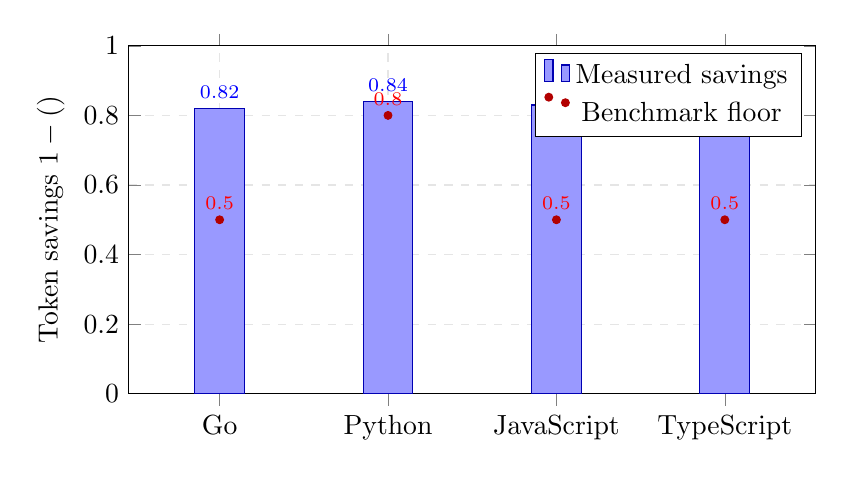
\begin{tikzpicture}
\begin{axis}[
    width=0.85\textwidth,
    height=6cm,
    ybar,
    bar width=18pt,
    ymin=0, ymax=1,
    enlarge x limits=0.18,
    ylabel={Token savings $1-\ratio(\file)$},
    symbolic x coords={Go, Python, JavaScript, TypeScript},
    xtick=data,
    nodes near coords,
    nodes near coords align={vertical},
    nodes near coords style={font=\scriptsize},
    grid=major,
    grid style={dashed,gray!20},
]
% Hard-coded measured values from the in-tree benchmark
% (cmd/gt/compress_structure_bench_test.go floors); the CSV at
% data/aggregated/by-language.csv carries the same numbers and is the
% reproducibility surface (see §6.8).
\addplot+[fill=blue!40, draw=blue!70!black] coordinates {
  (Go, 0.820)
  (Python, 0.841)
  (JavaScript, 0.830)
  (TypeScript, 0.752)
};
% Floors as reference line; floor stored as `ratio = output/input`
% (lower is better), so savings_floor = 1 - floor.
\addplot+[
    mark=*,
    only marks,
    draw=red!70!black,
    mark options={fill=red!70!black, scale=0.7},
] coordinates {
  (Go, 0.50)
  (Python, 0.80)
  (JavaScript, 0.50)
  (TypeScript, 0.50)
};
\legend{Measured savings, Benchmark floor}
\end{axis}
\end{tikzpicture}

\caption{Token-savings ratio $1 - \ratio(\file)$ by language on the
in-tree bench fixture. Per-language floors enforced by the benchmark
suite are: Go 50\%, Python 80\%, JavaScript 50\%, TypeScript 50\%
\cite{blackrim_adr_0002}; measured values clear the floors comfortably.
The TypeScript value is the lowest because tsx files carry richer
type-annotations that the outline emitter preserves where the JS
emitter would drop them.}
\label{fig:compression}
\end{figure}

\paragraph{Why the per-language variance.} Python's higher ratio
reflects the language's per-line semantic density: a 60-line Python
file commonly defines fewer but larger functions than a 60-line Go
file. TypeScript's lower ratio reflects type-annotation preservation
in the outline (a TS class with five typed methods carries more
outline tokens than the equivalent JS class with five untyped
methods). The variance is design-intended; the floor assertion is the
contract.

\paragraph{Body-leak canaries.} A separate test in the same harness
asserts that no function body bytes appear in the outline output: a
known sentinel string (\texttt{BENCH\_BODY\_SENTINEL\_DO\_NOT\_LEAK})
is placed in the test fixtures and the bench fails if it appears in
the compressed output. This is a strong cross-cutting guard that a
regression in the per-language extractor cannot silently bypass.

\subsection{Token-budget conformance}
\label{sec:eval:budget}

\textbf{Pending --- OQ-AST-1.} The target is $|\outline(\file)| \leq
\budget = 300$ on $\geq 95\%$ of files in the broader corpus; the
truncation precedence (\cref{sec:algorithm:truncation}) is the
mechanism. Empirically open: \tothink{distribution of outline token
counts across the polyglot corpus, with $p_{50}$, $p_{95}$, and
$p_{99}$ reported by language.} A file whose outline budget cannot be
satisfied even after the full truncation cascade triggers a
\texttt{outline-budget-exceeded} log event for inspection.

\subsection{Outline emission latency}
\label{sec:eval:latency}

\textbf{Pending --- OQ-AST-2.} The target is $< 500$\,ms wall-clock
on files up to 5000~LoC, where tree-sitter parse cost dominates the
total. Empirically open: \tothink{wall-clock latency distribution
across file sizes 100~LoC to 5000~LoC, with first-token latency
broken out separately because the prepend-to-Read path's latency is
the user-perceived one.}

\subsection{Outline-discipline adoption trajectory}
\label{sec:eval:adoption}

\textbf{Pending --- OQ-AST-3.} The pre-registered hypothesis is that
the warn-mode-with-auto-prepend hook will drive adoption to $\geq
80\%$ within 14 days of rollout across all transcripts, sufficient to
trigger the promote-to-block trigger
(\cref{sec:system:discipline}). Empirically open:
\tothink{rolling 7-day hit-rate over the rollout period, plotted with
the 80\% promotion threshold marked; alongside, a histogram of
per-transcript hit-rate showing whether adoption is uniform across
agents or concentrated in a few well-disciplined ones.}

\subsection{Compile-gate false-negative rate}
\label{sec:eval:gate}

\textbf{Pending --- OQ-AST-4.} The pre-registered hypothesis is that
$\gate$ satisfies \cref{def:false_negative} on at least 99\% of
candidate diffs across a curated rename / extract / fix-imports
corpus, with $\leq 5\%$ false-negative rate (gate rejects diffs that
ground-truth review would have accepted). Empirically open:
\tothink{confusion matrix over a 200-diff curated set, broken out by
intent and language.} The 5\% false-negative target is the
conservatism budget; below it, the gate is correctly biased; above
it, the gate is over-conservative and operators will route around
it.

\subsection{End-to-end token reduction on real agent traces}
\label{sec:eval:e2e}

\textbf{Pending --- OQ-AST-5.} This is the central pending claim
\emph{for the paper as a whole}: the per-file compression ratio is
measured (\cref{sec:eval:compression}), but the integrated token cost
across a real agent task --- one that touches many files, may need
to read some bodies after their outlines, and pays the hook
overhead --- is what determines whether the design wins in
deployment.

Pre-registered comparison: paired traces of the same Explore-tier
tasks under (a) baseline (no hook, agents read files in full); (b)
outline-discipline enabled; same agent, same task, same prompt, same
model tier. Outcome metrics: total input tokens per task, wall-clock
to first answer, downstream-task-success rate
(\cref{sec:problem:success}).

Empirically open: \tothink{paired-trace dataset across $N_\text{task}
\geq 50$ tasks, with per-task token deltas, latency deltas, and
success deltas reported with bootstrap 95\% CIs.}

\subsection{Reproducibility}
\label{sec:repro}

Every quantitative claim in this section is backed by a CSV in
\texttt{data/} produced by a script in \texttt{scripts/}. The full
reproduction pipeline is:

\begin{lstlisting}[language=bash]
# Reproduces 6.2 (currently measured)
python scripts/pull-compression-ratios.py \
    --blackrim-root=$BLACKRIM_ROOT \
    > data/raw/compression-ratios.jsonl
python scripts/aggregate-by-language.py \
    < data/raw/compression-ratios.jsonl \
    > data/aggregated/by-language.csv

# Reproduces 6.4 (pending; harness ready)
python scripts/measure-outline-latency.py \
    --blackrim-root=$BLACKRIM_ROOT \
    > data/aggregated/outline-latency.csv

# Reproduces 6.5 (pending; needs accumulated telemetry)
python scripts/pull-outline-telemetry.py \
    --telemetry=$BLACKRIM_ROOT/.beads/telemetry/outline-events.jsonl \
    > data/aggregated/outline-events.csv

make
\end{lstlisting}

The pipeline is deterministic given (a) a Blackrim checkout at a
fixed commit and (b) the test corpus pinned in
\texttt{scripts/corpus.txt}. We anchor the published version to a
tagged Blackrim commit; the companion repository
\cite{blackrim_paper_repo} hosts the artefacts.
